\section{Decision Boundary}
Neural network တွေကို သင်ပေးတဲ့နေရာမှာ သင်မဲ့ train dataset နဲ့ ရလာတဲ့ model ကို စမ်းသပ်မဲ့ test dataset တို့လိုပါတယ်။
အခုအောက်မှာ သင်ပေးမဲ့ train dataset ကိုကြည့်ရအောင်။

\begin{table}[h]
\centering
\begin{tabular}{ccc}
\hline
$x_1$ & $x_2$ & Class \\
\hline
1.0 & 1.0 & \tikz\draw[red, line width=1.5pt] (0,0) circle (4pt); \\
1.5 & 2.0 & \tikz\draw[red, line width=1.5pt] (0,0) circle (4pt); \\
2.0 & 1.5 & \tikz\draw[red, line width=1.5pt] (0,0) circle (4pt); \\
4.0 & 3.0 & \tikz\draw[blue, line width=2pt] (-4pt,-4pt) -- (4pt,4pt) (4pt,-4pt) -- (-4pt,4pt); \\
4.5 & 4.0 & \tikz\draw[blue, line width=2pt] (-4pt,-4pt) -- (4pt,4pt) (4pt,-4pt) -- (-4pt,4pt); \\
3.5 & 3.5 & \tikz\draw[blue, line width=2pt] (-4pt,-4pt) -- (4pt,4pt) (4pt,-4pt) -- (-4pt,4pt); \\
\hline
\end{tabular}
\caption{Training Dataset}
\end{table}

\noindent ဆိုလိုတာက input $x_1$ နဲ့ $x_2$ ပေးရင် အဖြေက \redcircle\ ဒါမှမဟုတ် \bluecross\ ဖြစ်မယ်။ အဲတာကို အောက်ကအတိုင်း graph ဆွဲကြည့်လိုရတယ်။

\begin{figure}[h]
\centering
    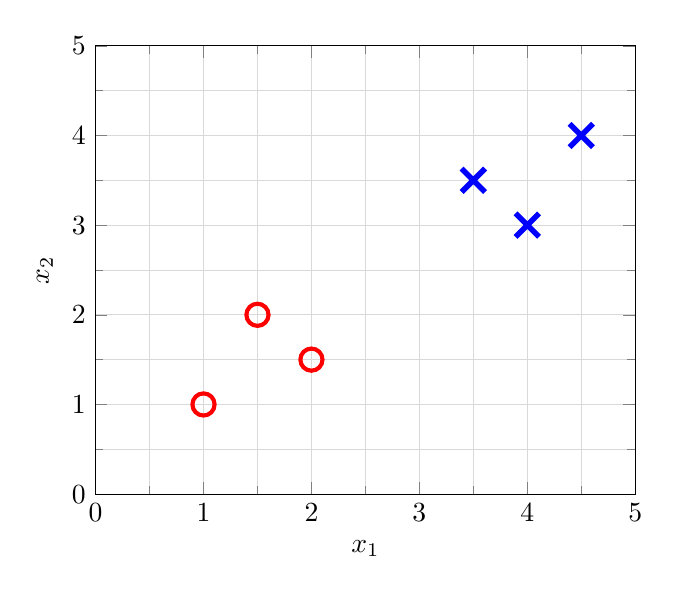
\begin{tikzpicture}
        \begin{axis}[
        xlabel={$x_1$}, ylabel={$x_2$},
        xmin=0, xmax=5, ymin=0, ymax=5,
        grid=both,
        grid style={line width=0.3pt, draw=gray!30},
        minor tick num=1,
        ]
        % Big Circle - Class 0
        \addplot[only marks, mark=o, mark size=4pt,
                line width=1.5pt, red]
        coordinates {(1,1)(1.5,2)(2,1.5)};

        % Big X - Class 1
        \addplot[only marks, mark=x, mark size=6pt,
                line width=2pt, blue]
        coordinates {(4,3)(4.5,4)(3.5,3.5)};
        \end{axis}
    \end{tikzpicture}
\caption{train dataset}
\end{figure}

\noindent အဲဒီ \redcircle\ နဲ့ \bluecross ကို ခွဲခြားပေးဖို့ မျဥ်းဆွဲကြည့်ရအောင်။ အောက်မှာ ဖြစ်နိုင်တဲ့ အဖြေတွေပေးထားတယ်။

\begin{figure}[h]
\centering

\begin{subfigure}[b]{0.45\textwidth}
\centering
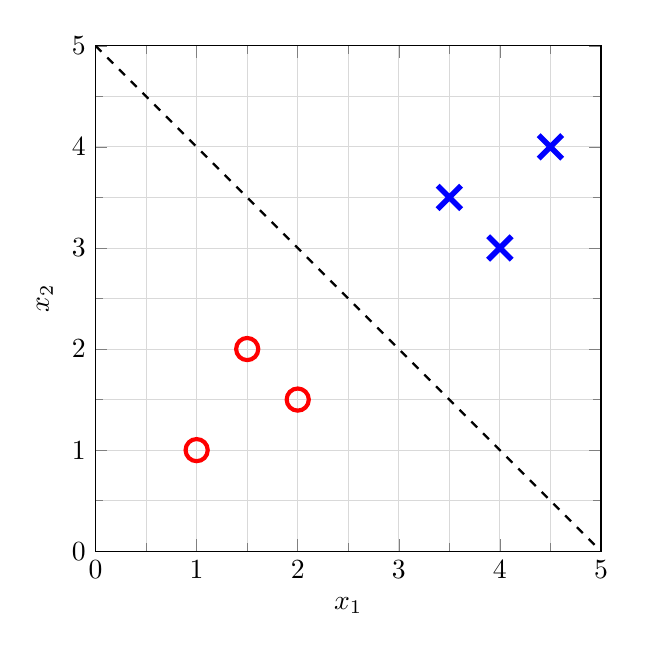
\begin{tikzpicture}
\begin{axis}[
  xlabel={$x_1$}, ylabel={$x_2$},
  xmin=0, xmax=5, ymin=0, ymax=5,
  grid=both,
  grid style={line width=0.3pt, draw=gray!30},
  minor tick num=1,
  width=8cm, height=8cm,
]
\addplot[only marks, mark=o, mark size=4pt,
         line width=1.5pt, red]
  coordinates {(1,1)(1.5,2)(2,1.5)};
\addplot[only marks, mark=x, mark size=6pt,
         line width=2pt, blue]
  coordinates {(4,3)(4.5,4)(3.5,3.5)};
% Decision boundary: x2 = x1
\addplot[domain=0:5, samples=2, thick, black, dashed]
  {-x + 5};
\end{axis}
\end{tikzpicture}
\end{subfigure}
\hfill
\begin{subfigure}[b]{0.45\textwidth}
\centering
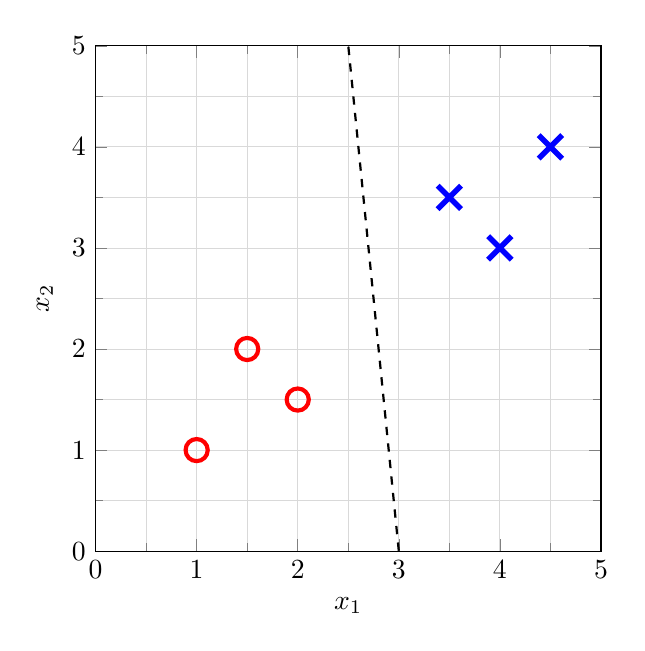
\begin{tikzpicture}
\begin{axis}[
  xlabel={$x_1$}, ylabel={$x_2$},
  xmin=0, xmax=5, ymin=0, ymax=5,
  grid=both,
  grid style={line width=0.3pt, draw=gray!30},
  minor tick num=1,
  width=8cm, height=8cm,
]
\addplot[only marks, mark=o, mark size=4pt,
         line width=1.5pt, red]
  coordinates {(1,1)(1.5,2)(2,1.5)};
\addplot[only marks, mark=x, mark size=6pt,
         line width=2pt, blue]
  coordinates {(4,3)(4.5,4)(3.5,3.5)};
% Decision boundary: x2 = -x1 + 5
\addplot[domain=0:5, samples=2, thick, black, dashed]
  {-10 * x + 30};
\end{axis}
\end{tikzpicture}
\end{subfigure}

\vspace{1em}

\begin{subfigure}[b]{0.45\textwidth}
\centering
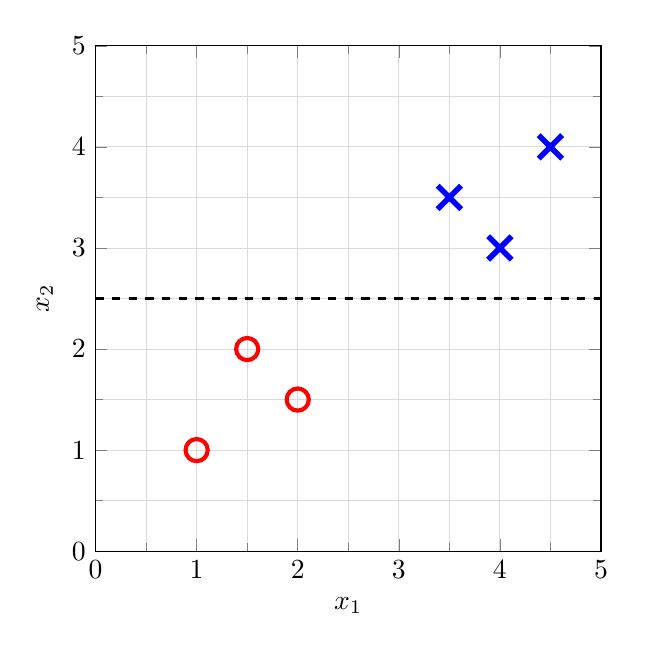
\begin{tikzpicture}
\begin{axis}[
  xlabel={$x_1$}, ylabel={$x_2$},
  xmin=0, xmax=5, ymin=0, ymax=5,
  grid=both,
  grid style={line width=0.3pt, draw=gray!30},
  minor tick num=1,
  width=8cm, height=8cm,
]
\addplot[only marks, mark=o, mark size=4pt,
         line width=1.5pt, red]
  coordinates {(1,1)(1.5,2)(2,1.5)};
\addplot[only marks, mark=x, mark size=6pt,
         line width=2pt, blue]
  coordinates {(4,3)(4.5,4)(3.5,3.5)};
\addplot[domain=0:5, samples=2, thick, black, dashed]
  {2.5};
\end{axis}
\end{tikzpicture}
\end{subfigure}
\hfill
\begin{subfigure}[b]{0.45\textwidth}
\centering
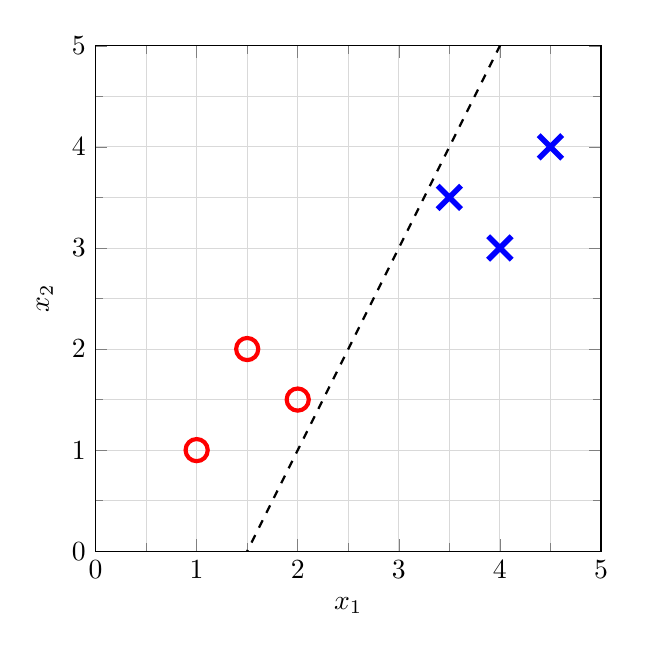
\begin{tikzpicture}
\begin{axis}[
  xlabel={$x_1$}, ylabel={$x_2$},
  xmin=0, xmax=5, ymin=0, ymax=5,
  grid=both,
  grid style={line width=0.3pt, draw=gray!30},
  minor tick num=1,
  width=8cm, height=8cm,
]
\addplot[only marks, mark=o, mark size=4pt,
         line width=1.5pt, red]
  coordinates {(1,1)(1.5,2)(2,1.5)};
\addplot[only marks, mark=x, mark size=6pt,
         line width=2pt, blue]
  coordinates {(4,3)(4.5,4)(3.5,3.5)};
% Decision boundary: x2 = -x1 + 5
\addplot[domain=0:5, samples=2, thick, black, dashed]
  {2 * x - 3};
\end{axis}
\end{tikzpicture}
\end{subfigure}

\caption{မှန်ကန်သော အဖြေများ}
\label{fig:decision_boundaries}
\end{figure}
\clearpage

အပေါ်က ၄ခုလုံးက ပေးထားတဲ့ ဒေတာတွေအားလုံးကို မှန်အောင်လုပ်ပေးနိုင်တဲ့ function တွေ ဖြစ်ကြတယ်။ အဲဒီ နယ်နိမိတ်နှစ်ခုကို ပိုင်းခြားပေးတာ မျဥ်းကို decision boundary လို့ခေါ်တယ်။ \\

\noindent ကျွန်တော်တို့ machine learning မှာ ပြဿနာတွေကို ဖြေရှင်းတဲ့ function တွေကို model လို့ခေါ်ကြတယ်။ အဲတာကြောင့် ဒီနေရာက စပြီး model လို့ပဲ ခေါ်ကြရအောင်။
အဲတာဆို အဲဒီ ၄ခုထဲမှာ ဘယ် model က အကောင်းဆုံးလဲ? \\

\noindent မြင်သာအောင် (intuition) ရအောင် ပြောရင် အလယ်ရောက်လေလေ ကောင်းလေပေါ့။ ဥပမာ \redcircle\ နဲ့ \bluecross\ တစ်ခုစီသာရှိခဲ့မယ်ဆိုရင် သူတို့နှစ်ခုရင် အလယ် ဗဟိုမှာ မျဥ်းဆွဲလိုက်ရင် ဘက်မလိုက် (unbiased) တော့ဘူးပေါ့။ ဒါကတော့ မြင်သာအောင် အလွယ်ပြောလိုက်တာ။ \\

\noindent ဘယ်ဟာမှ မရွေးခင် စမ်းသပ်မဲ့ test dataset ကို ကြည့်ကြရအောင်။

\begin{table}[h]
\centering
\begin{tabular}{ccc}
\hline
$x_1$ & $x_2$ & Class \\
\hline
2.5 & 4.0 & \tikz\draw[red, line width=1.5pt] (0,0) circle (4pt); \\
3.0 & 0.5 & \tikz\draw[blue, line width=2pt] (-4pt,-4pt) -- (4pt,4pt) (4pt,-4pt) -- (-4pt,4pt); \\
\hline
\end{tabular}
\caption{Test Dataset}
\end{table}

\begin{figure}
\centering

\begin{subfigure}[b]{0.45\textwidth}
\centering
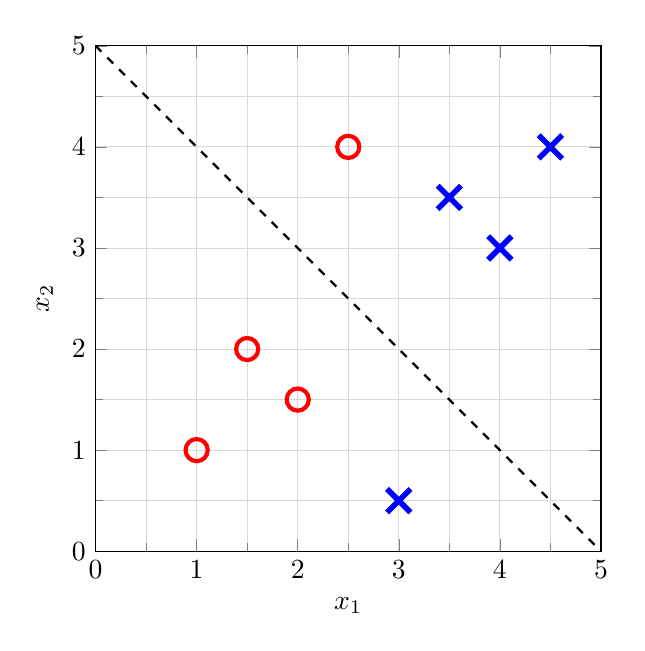
\begin{tikzpicture}
\begin{axis}[
  xlabel={$x_1$}, ylabel={$x_2$},
  xmin=0, xmax=5, ymin=0, ymax=5,
  grid=both,
  grid style={line width=0.3pt, draw=gray!30},
  minor tick num=1,
  width=8cm, height=8cm,
]
\addplot[only marks, mark=o, mark size=4pt,
         line width=1.5pt, red]
  coordinates {(1,1)(1.5,2)(2,1.5)(2.5,4.0)};
\addplot[only marks, mark=x, mark size=6pt,
         line width=2pt, blue]
  coordinates {(4,3)(4.5,4)(3.5,3.5)(3.0,0.5)};
% Decision boundary: x2 = x1
\addplot[domain=0:5, samples=2, thick, black, dashed]
  {-x + 5};
\end{axis}
\end{tikzpicture}
\end{subfigure}
\hfill
\begin{subfigure}[b]{0.45\textwidth}
\centering
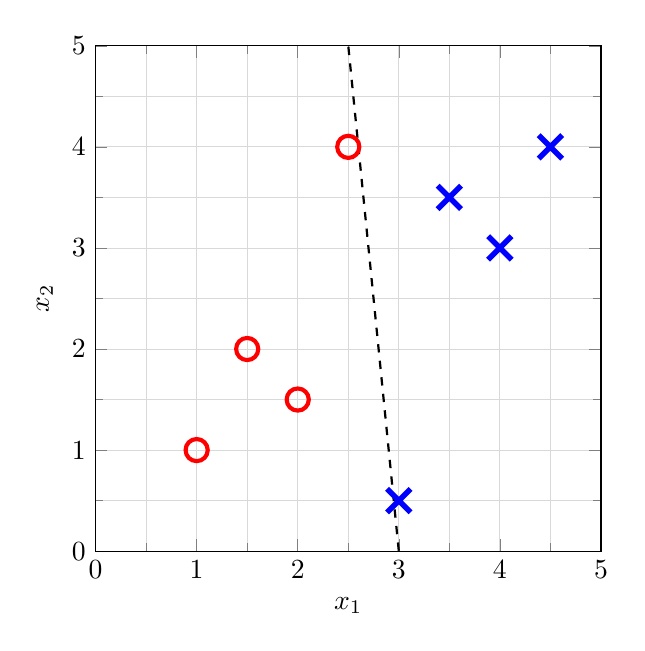
\begin{tikzpicture}
\begin{axis}[
  xlabel={$x_1$}, ylabel={$x_2$},
  xmin=0, xmax=5, ymin=0, ymax=5,
  grid=both,
  grid style={line width=0.3pt, draw=gray!30},
  minor tick num=1,
  width=8cm, height=8cm,
]
\addplot[only marks, mark=o, mark size=4pt,
         line width=1.5pt, red]
  coordinates {(1,1)(1.5,2)(2,1.5)(2.5,4.0)};
\addplot[only marks, mark=x, mark size=6pt,
         line width=2pt, blue]
  coordinates {(4,3)(4.5,4)(3.5,3.5)(3.0,0.5)};
% Decision boundary: x2 = -x1 + 5
\addplot[domain=0:5, samples=2, thick, black, dashed]
  {-10 * x + 30};
\end{axis}
\end{tikzpicture}
\end{subfigure}

\vspace{1em}

\begin{subfigure}[b]{0.45\textwidth}
\centering
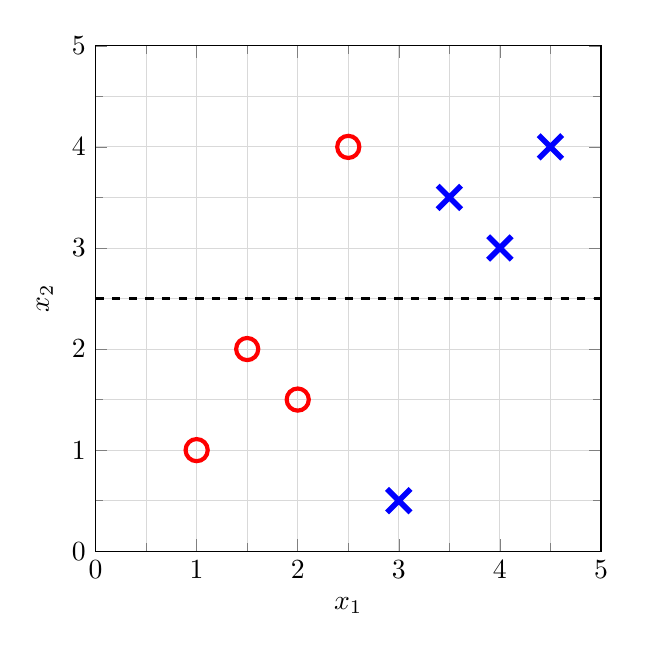
\begin{tikzpicture}
\begin{axis}[
  xlabel={$x_1$}, ylabel={$x_2$},
  xmin=0, xmax=5, ymin=0, ymax=5,
  grid=both,
  grid style={line width=0.3pt, draw=gray!30},
  minor tick num=1,
  width=8cm, height=8cm,
]
\addplot[only marks, mark=o, mark size=4pt,
         line width=1.5pt, red]
  coordinates {(1,1)(1.5,2)(2,1.5)(2.5,4.0)};
\addplot[only marks, mark=x, mark size=6pt,
         line width=2pt, blue]
  coordinates {(4,3)(4.5,4)(3.5,3.5)(3.0,0.5)};
\addplot[domain=0:5, samples=2, thick, black, dashed]
  {2.5};
\end{axis}
\end{tikzpicture}
\end{subfigure}
\hfill
\begin{subfigure}[b]{0.45\textwidth}
\centering
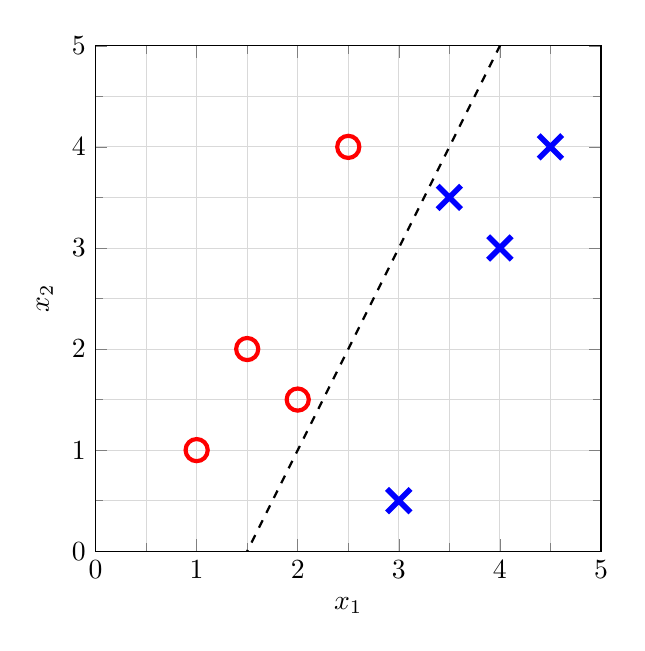
\begin{tikzpicture}
\begin{axis}[
  xlabel={$x_1$}, ylabel={$x_2$},
  xmin=0, xmax=5, ymin=0, ymax=5,
  grid=both,
  grid style={line width=0.3pt, draw=gray!30},
  minor tick num=1,
  width=8cm, height=8cm,
]
\addplot[only marks, mark=o, mark size=4pt,
         line width=1.5pt, red]
  coordinates {(1,1)(1.5,2)(2,1.5)(2.5,4.0)};
\addplot[only marks, mark=x, mark size=6pt,
         line width=2pt, blue]
  coordinates {(4,3)(4.5,4)(3.5,3.5)(3.0,0.5)};
% Decision boundary: x2 = -x1 + 5
\addplot[domain=0:5, samples=2, thick, black, dashed]
  {2 * x - 3};
\end{axis}
\end{tikzpicture}
\end{subfigure}

\caption{model တစ်ခုချင်းစီကို test dataset နဲ့ စမ်းထားပုံ}
\end{figure}
